Our results rely heavily on properties of the exponential family,
which we briefly review here.  A joint distribution $q(x,y)$ is a
member of the exponential family if the PDF / PMF is of the following
form,
\begin{equation}\label{eq:expfam}
  q(x,y) = h(x,y) \exp \left[\eta^TT(x,y)-A(\eta)\right].
\end{equation}
where $\eta$ are the \emph{natural parameters}, $h(x,y)$ is the \emph{base measure},
$T(x,y)$ the \emph{sufficient statistics}, and $A(\eta)$ is the
\emph{log-partition function}.
The exponential family includes many well-known distributions:
Bernoulli, Categorical, Poisson, Gamma, Gaussian, etc.  In addition to
the natural parameters $\eta$ each exponential family has an alternate
set of \emph{mean parameters} $\mu$, defined as the expected
sufficient statistics: $\mu = \mathbb{E}_q[ T(x,y) ]$. Mean parameters
play a key role in finding projections onto the exponential family, as
shown in Lemma~\ref{lemma:MMKL}.
\begin{lemma}[Moment Matching Projection]\label{lemma:MMKL}
  For any distribution $p(x,y)$ and exponential family $q(x,y)$ whose
  support includes that of $p$ the minimum Kullback-Leibler projection:
  \[
    q^* = \argmin_q \, \KL{p(X,Y)}{q(X,Y)}
  = \argmin_q \, \mathbb{E}_p\left[ \log \frac{p(X,Y)}{q(X,Y)} \right]
  \]
  is convex and the solution given by \emph{moment matching} conditions:
  $\mathbb{E}_p[T(X,Y)] = \mathbb{E}_q[ T(X,Y) ] = \mu^*$
\end{lemma}

%% Then \emph{moment matching} is
%% \begin{equation}\label{eq:mm}
%% \E_{p(x,y)}[T(x,y)]=\E_{q(x,y)}[T(x,y)]
%% \end{equation}
%% If we restrict ourselves to the exponential family, then moment matching minimizes 
%% KL divergence. 

The interested reader can consult the texts~\cite{bishop2006pattern,
murphy2012machine} for a proof of Lemma~\ref{lemma:MMKL} and more
details on the exponential family.  In this paper, we will focus on
Gaussian $q(x,y)$. \FIG\ref{fig:GMMex} shows an example of a GMM,
$p(x,y)$, with a moment matched variational Gaussian, $q(x,y)$ (left),
corresponding marginal projection (center), and resulting variational
estimators (right).
\begin{figure*}[!t]
  \centering \subfigure[Joint pdf
  contour]{ 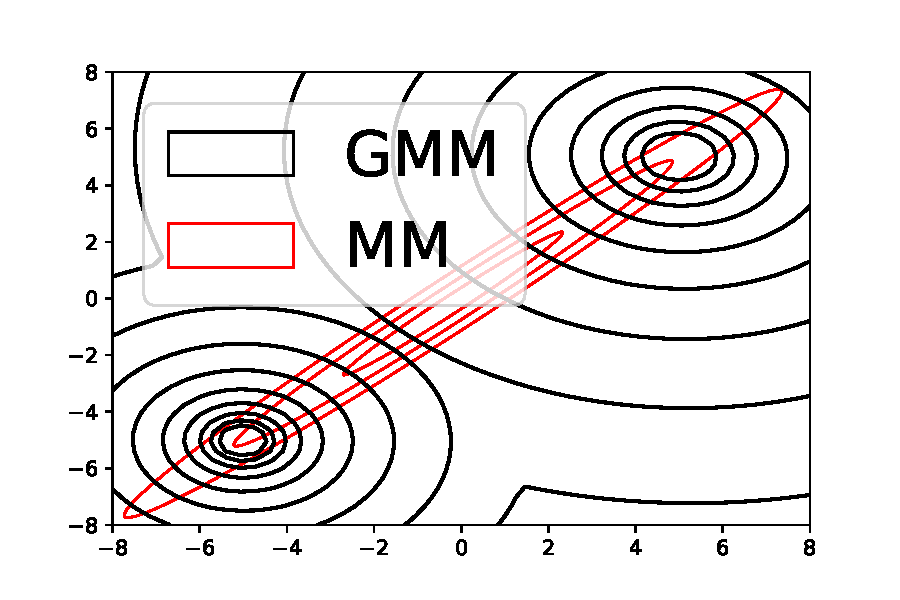
\includegraphics[width=.33\textwidth]{GMMContour.pdf}
  } \subfigure[Marginal
  pdf]{ 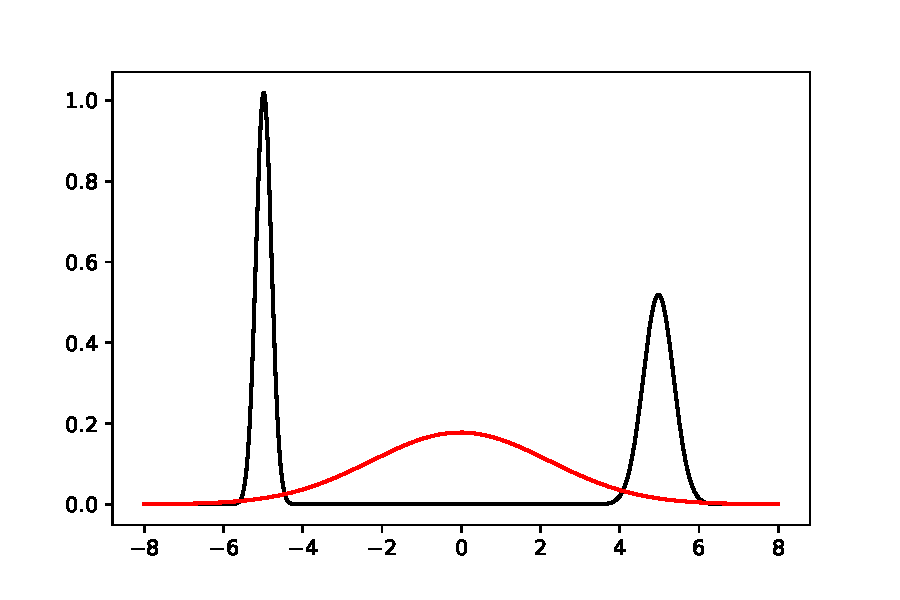
\includegraphics[width=.33\textwidth]{GMMpdf.pdf}
  } \subfigure[MI
  approximations]{ 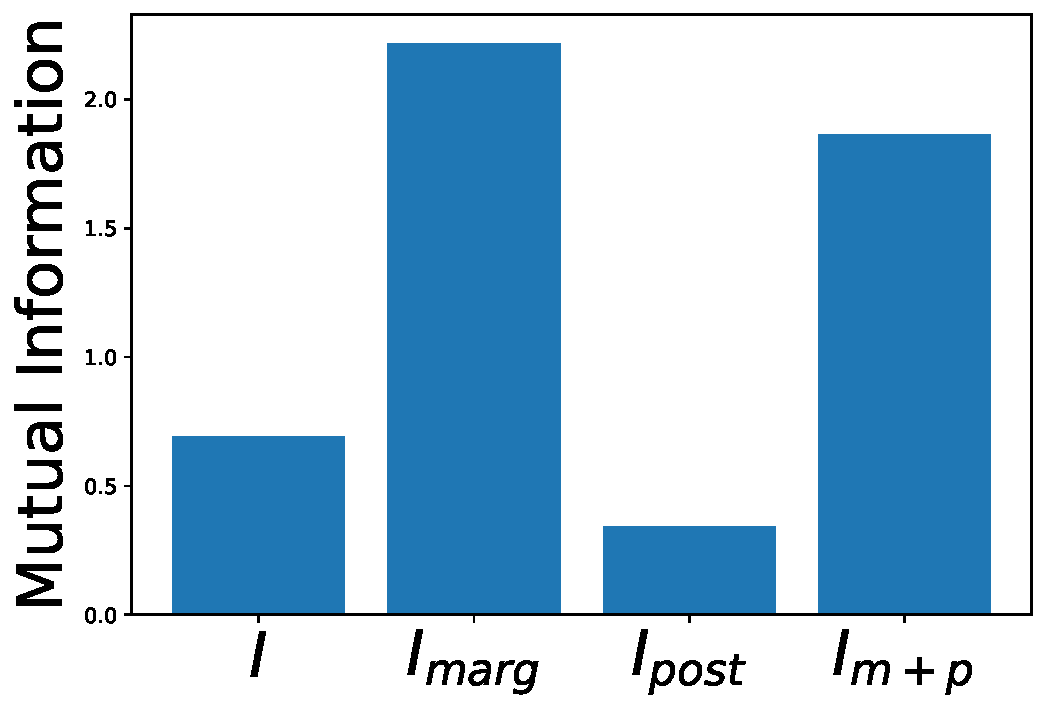
\includegraphics[width=.29\textwidth]{GMMbar.pdf}
  }

  \caption{\small\textbf{Moment Matched Gaussian Mixture Model} (a) A
  bimodal GMM $p$ overlaid with the moment matched Gaussian $q$ has
  its $.5$, $1$, and $1.5$ standard deviation level curves plotted on top in red. (b)
  The marginal PDF is plotted for the Gaussian mixture model and the
  moment matched Gaussian. (c) The true $I(X,Y)$ is shown with
  estimates $\Imarg$, $\Ipost$, and $\Iml$ are all plotted. Notice
  that $\Imarg \geq \Iml \geq \Ipost$.}

  \label{fig:GMMex}
\end{figure*}

%% includes There are many common distributions that fall into this family such as 
%% the Bernoulli distribution, Chi-squared distribution, Wishart distribution, 
%% Gaussian distribution, and many others. Let $q(x,y)$ be in the exponential 
%% family. 

%% The method we propose in this paper matching the moments of a variational 
%% distribution, $q(x,y)$, to those of $p(x,y)$. Our results rely on the properties
%% of the \emph{exponential family}.
%% \begin{definition}{Exponential Family}\\
%%   \emph{
%%   A distribution is a member of the exponential family if it's probability 
%%   density function can be expressed in the form
%%   \[f(x,y|\theta) = h(x,y) \exp \left[\eta(\theta)^TT(x,y)-A(\theta)\right]\]
%%   where $\theta$ are the parameters, $\eta(\theta)$ is the 
%%   natural parameters, $h(x,y)$ is the base measure, $T(x,y)$ is the sufficient 
%%   statistics, and $A(\theta)$ is the log-partition.}
%%   \end{definition}

